% Options for packages loaded elsewhere
\PassOptionsToPackage{unicode}{hyperref}
\PassOptionsToPackage{hyphens}{url}
\PassOptionsToPackage{dvipsnames,svgnames,x11names}{xcolor}
%
\documentclass[
  letterpaper,
  DIV=11,
  numbers=noendperiod]{scrartcl}

\usepackage{amsmath,amssymb}
\usepackage{iftex}
\ifPDFTeX
  \usepackage[T1]{fontenc}
  \usepackage[utf8]{inputenc}
  \usepackage{textcomp} % provide euro and other symbols
\else % if luatex or xetex
  \usepackage{unicode-math}
  \defaultfontfeatures{Scale=MatchLowercase}
  \defaultfontfeatures[\rmfamily]{Ligatures=TeX,Scale=1}
\fi
\usepackage{lmodern}
\ifPDFTeX\else  
    % xetex/luatex font selection
\fi
% Use upquote if available, for straight quotes in verbatim environments
\IfFileExists{upquote.sty}{\usepackage{upquote}}{}
\IfFileExists{microtype.sty}{% use microtype if available
  \usepackage[]{microtype}
  \UseMicrotypeSet[protrusion]{basicmath} % disable protrusion for tt fonts
}{}
\makeatletter
\@ifundefined{KOMAClassName}{% if non-KOMA class
  \IfFileExists{parskip.sty}{%
    \usepackage{parskip}
  }{% else
    \setlength{\parindent}{0pt}
    \setlength{\parskip}{6pt plus 2pt minus 1pt}}
}{% if KOMA class
  \KOMAoptions{parskip=half}}
\makeatother
\usepackage{xcolor}
\usepackage[top=20mm,left=20mm,right=20mm,bottom=20mm]{geometry}
\setlength{\emergencystretch}{3em} % prevent overfull lines
\setcounter{secnumdepth}{5}
% Make \paragraph and \subparagraph free-standing
\makeatletter
\ifx\paragraph\undefined\else
  \let\oldparagraph\paragraph
  \renewcommand{\paragraph}{
    \@ifstar
      \xxxParagraphStar
      \xxxParagraphNoStar
  }
  \newcommand{\xxxParagraphStar}[1]{\oldparagraph*{#1}\mbox{}}
  \newcommand{\xxxParagraphNoStar}[1]{\oldparagraph{#1}\mbox{}}
\fi
\ifx\subparagraph\undefined\else
  \let\oldsubparagraph\subparagraph
  \renewcommand{\subparagraph}{
    \@ifstar
      \xxxSubParagraphStar
      \xxxSubParagraphNoStar
  }
  \newcommand{\xxxSubParagraphStar}[1]{\oldsubparagraph*{#1}\mbox{}}
  \newcommand{\xxxSubParagraphNoStar}[1]{\oldsubparagraph{#1}\mbox{}}
\fi
\makeatother


\providecommand{\tightlist}{%
  \setlength{\itemsep}{0pt}\setlength{\parskip}{0pt}}\usepackage{longtable,booktabs,array}
\usepackage{calc} % for calculating minipage widths
% Correct order of tables after \paragraph or \subparagraph
\usepackage{etoolbox}
\makeatletter
\patchcmd\longtable{\par}{\if@noskipsec\mbox{}\fi\par}{}{}
\makeatother
% Allow footnotes in longtable head/foot
\IfFileExists{footnotehyper.sty}{\usepackage{footnotehyper}}{\usepackage{footnote}}
\makesavenoteenv{longtable}
\usepackage{graphicx}
\makeatletter
\def\maxwidth{\ifdim\Gin@nat@width>\linewidth\linewidth\else\Gin@nat@width\fi}
\def\maxheight{\ifdim\Gin@nat@height>\textheight\textheight\else\Gin@nat@height\fi}
\makeatother
% Scale images if necessary, so that they will not overflow the page
% margins by default, and it is still possible to overwrite the defaults
% using explicit options in \includegraphics[width, height, ...]{}
\setkeys{Gin}{width=\maxwidth,height=\maxheight,keepaspectratio}
% Set default figure placement to htbp
\makeatletter
\def\fps@figure{htbp}
\makeatother

\KOMAoption{captions}{tableheading}
\usepackage{sansmathfonts}
\usepackage[utf8]{inputenc}
\usepackage[T1]{fontenc}
\renewcommand*\familydefault{\sfdefault}
\makeatletter
\@ifpackageloaded{tcolorbox}{}{\usepackage[skins,breakable]{tcolorbox}}
\@ifpackageloaded{fontawesome5}{}{\usepackage{fontawesome5}}
\definecolor{quarto-callout-color}{HTML}{909090}
\definecolor{quarto-callout-note-color}{HTML}{0758E5}
\definecolor{quarto-callout-important-color}{HTML}{CC1914}
\definecolor{quarto-callout-warning-color}{HTML}{EB9113}
\definecolor{quarto-callout-tip-color}{HTML}{00A047}
\definecolor{quarto-callout-caution-color}{HTML}{FC5300}
\definecolor{quarto-callout-color-frame}{HTML}{acacac}
\definecolor{quarto-callout-note-color-frame}{HTML}{4582ec}
\definecolor{quarto-callout-important-color-frame}{HTML}{d9534f}
\definecolor{quarto-callout-warning-color-frame}{HTML}{f0ad4e}
\definecolor{quarto-callout-tip-color-frame}{HTML}{02b875}
\definecolor{quarto-callout-caution-color-frame}{HTML}{fd7e14}
\makeatother
\makeatletter
\@ifpackageloaded{caption}{}{\usepackage{caption}}
\AtBeginDocument{%
\ifdefined\contentsname
  \renewcommand*\contentsname{Table des matières}
\else
  \newcommand\contentsname{Table des matières}
\fi
\ifdefined\listfigurename
  \renewcommand*\listfigurename{Liste des Figures}
\else
  \newcommand\listfigurename{Liste des Figures}
\fi
\ifdefined\listtablename
  \renewcommand*\listtablename{Liste des Tables}
\else
  \newcommand\listtablename{Liste des Tables}
\fi
\ifdefined\figurename
  \renewcommand*\figurename{Figure}
\else
  \newcommand\figurename{Figure}
\fi
\ifdefined\tablename
  \renewcommand*\tablename{Table}
\else
  \newcommand\tablename{Table}
\fi
}
\@ifpackageloaded{float}{}{\usepackage{float}}
\floatstyle{ruled}
\@ifundefined{c@chapter}{\newfloat{codelisting}{h}{lop}}{\newfloat{codelisting}{h}{lop}[chapter]}
\floatname{codelisting}{Listing}
\newcommand*\listoflistings{\listof{codelisting}{Liste des Listings}}
\makeatother
\makeatletter
\makeatother
\makeatletter
\@ifpackageloaded{caption}{}{\usepackage{caption}}
\@ifpackageloaded{subcaption}{}{\usepackage{subcaption}}
\makeatother

\ifLuaTeX
\usepackage[bidi=basic]{babel}
\else
\usepackage[bidi=default]{babel}
\fi
\babelprovide[main,import]{french}
% get rid of language-specific shorthands (see #6817):
\let\LanguageShortHands\languageshorthands
\def\languageshorthands#1{}
\ifLuaTeX
  \usepackage{selnolig}  % disable illegal ligatures
\fi
\usepackage{bookmark}

\IfFileExists{xurl.sty}{\usepackage{xurl}}{} % add URL line breaks if available
\urlstyle{same} % disable monospaced font for URLs
\hypersetup{
  pdftitle={Fusion et fission nucléaire},
  pdflang={fr},
  colorlinks=true,
  linkcolor={blue},
  filecolor={Maroon},
  citecolor={Blue},
  urlcolor={Blue},
  pdfcreator={LaTeX via pandoc}}


\title{Fusion et fission nucléaire}
\author{}
\date{}

\begin{document}
\maketitle


\includegraphics[width=\textwidth]{./figures/ff/sun.png}
\newpage

\section{La relation d'Einstein}\label{la-relation-deinstein}

\subsection{Introduction}\label{introduction}

Regardons la vidéo suivante de ScienceEtonnante:

\begin{figure}[H]

{\centering 
\includegraphics[width=0.2\textwidth,height=\textheight]{figures/ff/video-mc2.pdf}

}

\caption{QR-code de la vidéo}

\end{figure}%

Réponds aux questions suivantes:

\begin{enumerate}
\def\labelenumi{\arabic{enumi}.}
\tightlist
\item
  Quelle est l'équation la plus connue de la physique?
\end{enumerate}

\vspace{1cm}

\begin{enumerate}
\def\labelenumi{\arabic{enumi}.}
\setcounter{enumi}{1}
\tightlist
\item
  Comment devrait-on écrie cette équation?
\end{enumerate}

\vspace{1cm}

\begin{enumerate}
\def\labelenumi{\arabic{enumi}.}
\setcounter{enumi}{2}
\tightlist
\item
  Quelles quantités varient simultanément?
\end{enumerate}

\vspace{1cm}

\begin{enumerate}
\def\labelenumi{\arabic{enumi}.}
\setcounter{enumi}{5}
\tightlist
\item
  Dans l'équation d'Einstein, que représente \(m\)?
\end{enumerate}

\vspace{1cm}

\begin{enumerate}
\def\labelenumi{\arabic{enumi}.}
\setcounter{enumi}{5}
\tightlist
\item
  Dans l'équation d'Einstein, que représente \(E\)?
\end{enumerate}

\vspace{1cm}

\begin{enumerate}
\def\labelenumi{\arabic{enumi}.}
\setcounter{enumi}{6}
\tightlist
\item
  Pourquoi dit-on qu'il y a une perte de masse dans un atome
  d'hydrogène?
\end{enumerate}

\vspace{3cm}

\begin{enumerate}
\def\labelenumi{\arabic{enumi}.}
\setcounter{enumi}{7}
\tightlist
\item
  De quoi est composé un noyau d'hélium?
\end{enumerate}

\vspace{1cm}

\begin{enumerate}
\def\labelenumi{\arabic{enumi}.}
\setcounter{enumi}{8}
\tightlist
\item
  Peut-on dire qu'il est possible de transformer de la masse en énergie?
\end{enumerate}

\vspace{4cm}

\subsection{La relation d'Einstein}\label{la-relation-deinstein-1}

C'est en 1905 qu'Einstein publia l'équation \(E=mc^2\), sur base de
nombreux travaux d'autres scientifiques qui avaient déjà observé un lien
entre l'énergie et la masse dans des situations particulières.

Décortiquons cette équation:

\begin{itemize}
\tightlist
\item
  cette équation parle de deux attributs \(E\) et \(m\) d'un corps
  supposé au repos;
\item
  la lettre \(m\) fait référence à la masse de ce corps (au repos!),
  exprimée en kilogrammes \(\text{kg}\);
\item
  la lettre \(E\) fait référence à l'énergie totale de ce corps (au
  repos!), exprimée en joules \(J\);
\item
  la lettre \(c\) fait référence à la vitesse de la lumière dans le
  vide, qui est une constante universelle et vaut environ
  \(300 000\text{km/s}=3\cdot 10^8\text{m/s}\).
\end{itemize}

Dans cette équation, la masse est une mesure de la résistance du corps à
se mettre en mouvement et n'est donc pas une mesure de la quantité de
matière.

Comment interpréter cette équation? Elle nous dit qu'une variation de
l'énergie d'un corps au repos correspond à une variation de la masse de
ce corps. De plus, le facteur \(c^2\) qui lie ces variations entre
énergie et masse fait qu'une variation de l'énergie correspond à une
variation sensiblement plus petite de la masse (une variation environ
\(10^{17}\) fois plus petite).

Voici un tableau donnant différentes variations d'énergie et la
variation de masse correspondante:

\begin{longtable}[]{@{}
  >{\raggedright\arraybackslash}p{(\columnwidth - 6\tabcolsep) * \real{0.2000}}
  >{\raggedright\arraybackslash}p{(\columnwidth - 6\tabcolsep) * \real{0.3000}}
  >{\raggedright\arraybackslash}p{(\columnwidth - 6\tabcolsep) * \real{0.2000}}
  >{\raggedright\arraybackslash}p{(\columnwidth - 6\tabcolsep) * \real{0.3000}}@{}}
\toprule\noalign{}
\begin{minipage}[b]{\linewidth}\raggedright
Énergie (J)
\end{minipage} & \begin{minipage}[b]{\linewidth}\raggedright
Exemple
\end{minipage} & \begin{minipage}[b]{\linewidth}\raggedright
Masse (kg)
\end{minipage} & \begin{minipage}[b]{\linewidth}\raggedright
Exemple
\end{minipage} \\
\midrule\noalign{}
\endhead
\bottomrule\noalign{}
\endlastfoot
\(2,11 \cdot 10^{18}\) & Consommation totale d'énergie de la Belgique en
1 an & \(23,5\) & un enfant de 8 ans \\
\(9 \cdot 10^{10}\) & Énergie consommée par une personne en un an &
\(1 \cdot 10^{-6}\) & un moustique \\
\(3,8 \cdot 10^{26}\) & Énergie émise par le Soleil en une seconde &
\(4,2 \cdot 10^9\) & la grande pyramide de Gizeh \\
\(1 \cdot 10^6\) & Énergie cinétique d'une voiture à 100 km/h &
\(1,11 \cdot 10^{-11}\) & dix cellules \\
\(8,368 \cdot 10^6\) & Énergie d'un repas de 2000 kcal &
\(9,3 \cdot 10^{-11}\) & un dixième de grain de sable \\
\(1\) & Énergie pour soulever une pomme d'un mètre &
\(1,11 \cdot 10^{-17}\) & une bactérie \\
\(2,9288 \cdot 10^6\) & Énergie dépensée lors d'une course de 10 km &
\(3,26 \cdot 10^{-11}\) & 30 cellules \\
\end{longtable}

\subsection{Le défaut de masse dans la formation de
noyaux}\label{le-duxe9faut-de-masse-dans-la-formation-de-noyaux}

Nous avons vu dans la vidéo que la masse d'un noyau d'hélium n'est pas
égale à la somme des masses des 4 nucléons qui le compose, à cause de
l'énergie nécessaire pour la création de ce noyau. Analysons un autre
exemple: celui du noyau d'un isotope de l'hydrogène, le deutérium.

Le noyau de cet isotope contient un proton et un neutron.

\begin{figure}[H]

{\centering 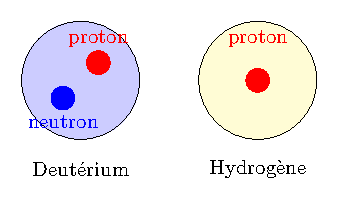
\includegraphics[width=0.6\textwidth,height=\textheight]{figures/ff/fig1.pdf}

}

\caption{Représentation des noyaux de deuterium et de l'hydrogène}

\end{figure}%

Voici un tableau résummant les valeurs des masses et du défaut de masse,
ainsi que l'énergie correspondant à ce défaut.

\begin{longtable}[]{@{}
  >{\raggedright\arraybackslash}p{(\columnwidth - 2\tabcolsep) * \real{0.7000}}
  >{\raggedright\arraybackslash}p{(\columnwidth - 2\tabcolsep) * \real{0.3000}}@{}}
\toprule\noalign{}
\begin{minipage}[b]{\linewidth}\raggedright
Élément
\end{minipage} & \begin{minipage}[b]{\linewidth}\raggedright
Valeur
\end{minipage} \\
\midrule\noalign{}
\endhead
\bottomrule\noalign{}
\endlastfoot
Masse du proton (p) & \(1.67262 \times 10^{-27}\text{kg}\) \\
Masse du neutron (n) & \(1.67493 \times 10^{-27}\text{kg}\) \\
Somme des masses (p + n) & \(3.34755 \times 10^{-27}\text{kg}\) \\
Masse réelle du deutérium & \(3.34449 \times 10^{-27}\text{kg}\) \\
Défaut de masse & \(3.06 \times 10^{-30}\text{kg}\) \\
Énergie de liaison & \(2.75 \times 10^{-13}\) J \\
\end{longtable}

Un noyau de deutérium est créé à partir d'hydrogène lorsqu'un proton
capture un neutron. Ce processus peut se produire naturellement, mais à
un taux très faible, ou être provoqué artificiellement dans des
réacteurs nucléaires. L'équation de formation du deutérium peut s'écrire
:

\[
^1_1\text{H} + ^1_0\text{n} \rightarrow ^2_1\text{H} + \gamma
\]

Cette réaction libère de l'énergie sous forme de rayonnement gamma,
correspondant au défaut de masse.

\section{Les réactions nucléaires}\label{les-ruxe9actions-nucluxe9aires}

\subsection{Introduction}\label{introduction-1}

Regardons la vidéo suivante de ScienceEtonnante:

\begin{figure}[H]

{\centering 
\includegraphics[width=0.2\textwidth,height=\textheight]{figures/ff/video-nucl.pdf}

}

\caption{QR-code de la vidéo}

\end{figure}%

Réponds aux questions suivantes:

\begin{enumerate}
\def\labelenumi{\arabic{enumi}.}
\tightlist
\item
  peut-on produire de l'énergie?
\end{enumerate}

\vspace{4cm}

\begin{enumerate}
\def\labelenumi{\arabic{enumi}.}
\setcounter{enumi}{1}
\tightlist
\item
  de quoi a-t-on besoin pour faire une fission?
\end{enumerate}

\vspace{2cm}

\begin{enumerate}
\def\labelenumi{\arabic{enumi}.}
\setcounter{enumi}{2}
\tightlist
\item
  combien y a-t-il de neutrons dans un noyau de magnésium 26?
\end{enumerate}

\vspace{1cm}

\begin{enumerate}
\def\labelenumi{\arabic{enumi}.}
\setcounter{enumi}{3}
\tightlist
\item
  que doit-il se produire pour qu'une réaction de fission puisse
  s'auto-entretenir?
\end{enumerate}

\vspace{4cm}

\begin{enumerate}
\def\labelenumi{\arabic{enumi}.}
\setcounter{enumi}{4}
\tightlist
\item
  quels noyaux permettent de créer des réactions de fission qui
  s'auto-entretiennent?
\end{enumerate}

\vspace{2cm}

\begin{enumerate}
\def\labelenumi{\arabic{enumi}.}
\setcounter{enumi}{5}
\item
  quels noyaux doit-on utiliser pour produire un noyau d'hélium par
  fusion? \vspace{1cm}
\item
  qu'est-ce que la barrière énergétique? \vspace{3cm}
\end{enumerate}

\subsection{La fission}\label{la-fission}

\begin{tcolorbox}[enhanced jigsaw, titlerule=0mm, leftrule=.75mm, title={Fission nucléaire}, opacityback=0, colbacktitle=quarto-callout-note-color!10!white, rightrule=.15mm, toptitle=1mm, coltitle=black, bottomtitle=1mm, left=2mm, colframe=quarto-callout-note-color-frame, colback=white, toprule=.15mm, bottomrule=.15mm, breakable, arc=.35mm, opacitybacktitle=0.6]

La fission nucléaire est une réaction selon laquelle un noyau lourd se
sépare en deux autres noyaux, plus légers, sous l'impact d'un neutron
lent. Cette réaction est accompagnée par l'émission de plusieurs
neutrons (en général 2 ou 3) et d'un dégagement d'énergie.

\end{tcolorbox}

Dans les centrales nucléaires, les réactions de fission sont causée par
bombardement d'un noyau lourd par un neutron. Voici deux exemples de
réaction par fission:

\[
 ^{235}_{92}\text{U} + ^1_0\text{n} \rightarrow ^{236}_{92}\text{U}\rightarrow ^{95}_{38}\text{Sr} + ^{139}_54\text{Xe} + 2 ^1_0\text{n} + 3,2 \cdot 10^{-11}\text{J}
 \]

\[
 ^{235}_{92}\text{U} + ^1_0\text{n} \rightarrow ^{236}_{92}\text{U}\rightarrow ^{92}_{36}\text{Kr} + ^{141}_{56}\text{Ba} + 3 ^1_0\text{n} + 3,2 \cdot 10^{-11}\text{J}
 \]

Pour chacune de ces deux réactions, l'énergie correspond au défaut de
masse entre les produits de fission et le noyau de départ. Pour la
réaction de fission de l'uranium-235, l'énérgie totale dégagée en
moyenne est de \(3,2 \cdot 10^{-11}\text{J}\). Cette énergie se
décompose de la manière suivante:

\begin{figure}[H]

{\centering 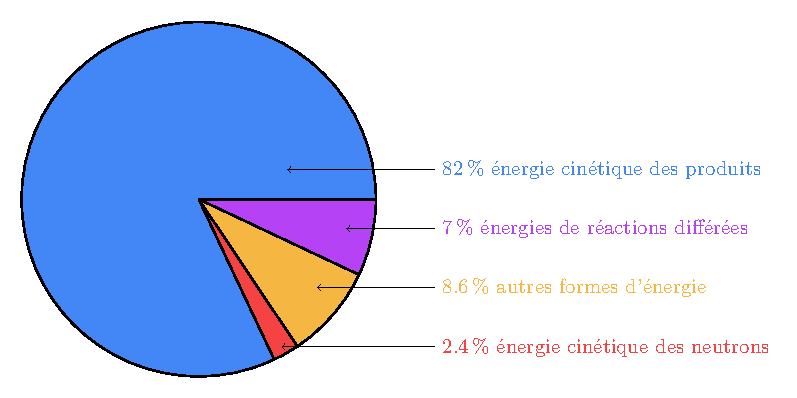
\includegraphics[width=0.8\textwidth,height=\textheight]{figures/ff/fig2.pdf}

}

\caption{Énergie d'une réaction de fission de l'uranium-235}

\end{figure}%

L'énergie récupérable par une centrale nucléaire est de l'ordre de
\(95\%\), c'est-à-dire environ \(3,04 \cdot 10^{-11}\text{J}\). Ce
nombre semble ridiculement petit mais est en fait énorme à grande
échelle. Voici un tableau comparant les différentes manière de produire
l'électricité nécessaire pour alimenter une maison pendant un an:

\begin{longtable}[]{@{}ll@{}}
\toprule\noalign{}
Source d'énergie & Quantité nécessaire pour 1 an \\
\midrule\noalign{}
\endhead
\bottomrule\noalign{}
\endlastfoot
Uranium (fission) & 17 g \\
Charbon (combustion) & 330 kg \\
Gaz naturel (combustion) & 300 m³ \\
Pétrole (combustion) & 270 litres \\
Panneaux solaires & envirion 15 panneaux solaires \\
\end{longtable}

\subsection{La fusion}\label{la-fusion}

\begin{tcolorbox}[enhanced jigsaw, titlerule=0mm, leftrule=.75mm, title={Fusion nucléaire}, opacityback=0, colbacktitle=quarto-callout-note-color!10!white, rightrule=.15mm, toptitle=1mm, coltitle=black, bottomtitle=1mm, left=2mm, colframe=quarto-callout-note-color-frame, colback=white, toprule=.15mm, bottomrule=.15mm, breakable, arc=.35mm, opacitybacktitle=0.6]

La fusion nucléaire est une réaction selon laquelle des noyaux légers
fusionnent pour former des noyaux plus lourds. Cette réaction
s'accompagne d'une libération importante d'énergie.

\end{tcolorbox}

Voici deux exemples de réactions de fusion nucléaire, faisant intervenir
des isotopes de l'hydrogène:

\begin{enumerate}
\def\labelenumi{\arabic{enumi}.}
\tightlist
\item
  Fusion deutérium-deutérium \[
  ^2_1 \text{H}+^2_1\text{H}\to ^3_2\text{He}+^1_0\text{n}+5,24 × 10^{-13}\text{J}
  \]
\end{enumerate}

Dans cette réaction, l'énergie dégagée correspond aux énergies
cinétiques des produits (75\% pour le neutron et 25\% pour le noyau
d'hélium-3).

\begin{enumerate}
\def\labelenumi{\arabic{enumi}.}
\setcounter{enumi}{1}
\tightlist
\item
  Fusion deutérium-tritium (isotope de l'hydrogène avec 2 neutrons) \[
  ^2_1\text{H}+^3_1\text{H}\to ^4_2\text{He}+^1_0\text{n}+2,82 × 10^{-12}\text{J}
  \]
\end{enumerate}

Dans cette réaction, l'énergie dégagée correspond aux énergies
cinétiques des produits (80\% pour le neutron et 20\% pour le noyau
d'hélium-4).

Voici un tableau comparant les différentes réactions nucléaires, pour
alimenter en électricité une maison pendant un an.

\begin{longtable}[]{@{}lll@{}}
\toprule\noalign{}
Type de réaction & Éléments requis & Masse nécessaire pour 1 an \\
\midrule\noalign{}
\endhead
\bottomrule\noalign{}
\endlastfoot
\textbf{Fission} & Uranium-235 & 17 g \\
\textbf{Fusion D-T} & Deutérium + Tritium & 0,04 g \\
\textbf{Fusion D-D} & Deutérium & 0,06 g \\
\end{longtable}

Malheureusement, il n'est pas encore possible de réaliser de manière
fiable et exploitable une fusion nucléaire. Les centrales à fusion sont
encore en développement et présentent de nombreux défis. Un projet
mondial, exécuté en France, essaye de développer un réacteur à fusion
nucléaire: c'est le projet ITER. Voici une courte vidéo qui l'explique.

\begin{figure}[H]

{\centering 
\includegraphics[width=0.15\textwidth,height=\textheight]{figures/ff/video-iter.pdf}

}

\caption{QR-code de la vidéo}

\end{figure}%

La fusion nucléaire est un phénomène fondamental qui alimente le Soleil.
Cette réaction est la source principale de l'énergie solaire dont nous
bénéficions sur Terre. Le processus de fusion dans le Soleil est si
intense qu'il entraîne une perte de masse significative : environ 4,2
millions de tonnes par seconde sont converties en énergie.

Les réactions nucléaires au cœur du Soleil sont complexes et variées,
formant des chaînes de réactions interconnectées. La chaîne
proton-proton (PP) est la plus importante, représentant la majorité des
réactions de fusion solaire. À titre d'illustration, voici les étapes
principales d'une partie de la chaîne, qui débute par la fusion de deux
noyaux d'hydrogène-1:

\begin{figure}[H]

{\centering 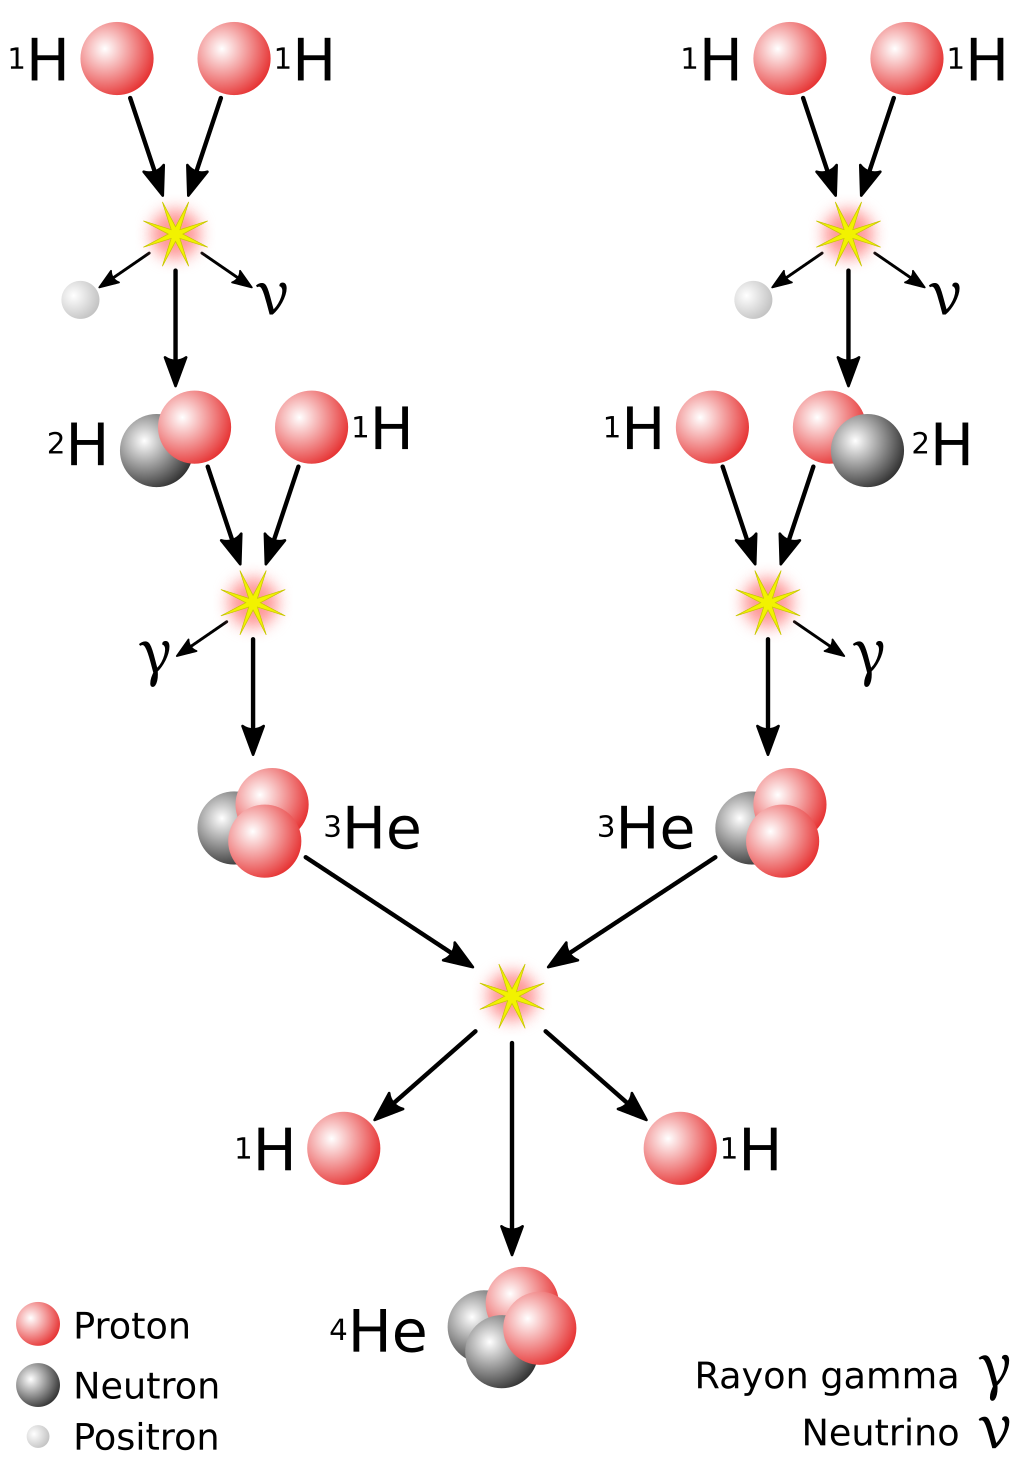
\includegraphics[width=0.45\textwidth,height=\textheight]{figures/ff/soleil.png}

}

\caption{Source:
\url{https://fr.wikipedia.org/wiki/Chaîne_proton-proton}}

\end{figure}%

Ces réactions se produisent dans des conditions extrêmes de température
(environ 15 millions de degrés Celsius) et de pression (la pression au
coeur du Soleil est égale à 200 milliards de fois la pression
atmosphérique terrestre) au coeur du Soleil.




\end{document}
